%------------------------------------------------------------------------------
% Template file for the submission of papers to IUCr journals in LaTeX2e
% using the iucr document class
% Copyright 1999-2007 International Union of Crystallography
% Version 1.3 (15 May 2007)
%------------------------------------------------------------------------------

\documentclass[preprint]{iucr}              % DO NOT DELETE THIS LINE
%%\documentclass{iucr}              % DO NOT DELETE THIS LINE
\usepackage{url}
\usepackage{graphicx}


     %-------------------------------------------------------------------------
     % Information about the type of paper
     %-------------------------------------------------------------------------
     \paperprodcode{a000000}      % Replace with production code if known
     \paperref{xx9999}            % Replace xx9999 with reference code if known
     \papertype{FA}               % Indicate type of article
                                  %   FA - research papers (full article)
                                  %   SC - short communications
                                  %   LA - lead article
                                  %   FE - feature articles
                                  %   GC - structural genomics communications
                                  %   NC - nucleic acid structure communications
                                  %   PC - protein structure communications
                                  %   XC - crystallization communications
                                  % (Following categories rarely in LaTeX)
                                  %   AA - abstracts
                                  %   AD - addenda and errata
                                  %   BC - books received
                                  %   BR - book reviews
                                  %   CA - cif applications
                                  %   CE - current events
                                  %   CI - inorganic compounds
                                  %   CM - metal-organic compounds
                                  %   CN - cryocrystallography papers
                                  %   CO - organic compounds
                                  %   CP - computer programs
                                  %   CR - crystallographers
                                  %   CS - scientific comment
                                  %   ED - editorial
                                  %   EI - inorganic compounds
                                  %   EM - metal-organic compounds
                                  %   EO - organic compounds
                                  %   FI - inorganic compounds
                                  %   FM - metal-organic compounds
                                  %   FO - organic compounds
                                  %   IP - issue preface
                                  %   IU - iucr
                                  %   LE - letters to the editor
                                  %   LN - laboratory notes
                                  %   ME - forthcoming meetings/short courses
                                  %   MR - meeting reports
                                  %   NN - notes and news
                                  %   NP - new commercial products
                                  %   OB - obituaries
                                  %   SR - software reviews
                                  %   TE - teaching and education

     \paperlang{english}          % Can be english, french, german or russian
     %-------------------------------------------------------------------------
     % Information about journal to which submitted
     %-------------------------------------------------------------------------
     \journalcode{J}              % Indicate the journal to which submitted
                                  %   A - Acta Crystallographica Section A
                                  %   B - Acta Crystallographica Section B
                                  %   C - Acta Crystallographica Section C
                                  %   D - Acta Crystallographica Section D
                                  %   E - Acta Crystallographica Section E
                                  %   F - Acta Crystallographica Section F
                                  %   J - Journal of Applied Crystallography
                                  %   S - Journal of Synchrotron Radiation
          %--------------------------------------------------------------------
          % The following entries will be changed as required by editorial staff
          %--------------------------------------------------------------------
     \journalyr{2007}
     \journaliss{1}
     \journalvol{63}
     \journalfirstpage{000}
     \journallastpage{000}
     \journalreceived{0 XXXXXXX 0000}
     \journalaccepted{0 XXXXXXX 0000}
     \journalonline{0 XXXXXXX 0000}

\begin{document}                  % DO NOT DELETE THIS LINE

     %-------------------------------------------------------------------------
     % The introductory (header) part of the paper
     %-------------------------------------------------------------------------

     % The title of the paper. Use \shorttitle to indicate an abbreviated title
     % for use in running heads (you will need to uncomment it).

\title{Integration of CBF, NeXus and HDF5}
\shorttitle{Integration of CBF, NeXus and HDF5}

     % Authors' names and addresses. Use \cauthor for the main (contact) author.
     % Use \author for all other authors. Use \aff for authors' affiliations.
     % Use lower-case letters in square brackets to link authors to their
     % affiliations; if there is only one affiliation address, remove the [a].

\cauthor[a]{Herbert J}{Bernstein}{yayahjb@gmail.com}{}
\author[b]{Graeme}{Winter}
\author[b]{Tobias S.}{Richter}
\author[b]{Mark}{Basham}
\author[b]{James}{Parkhurst}
\author[c]{}{NeXus International Advisory Committee}
\author[d]{}{Committee on the Maintenance of the CIF Standard}

\aff[a]{Department of Mathematics and Computer Science, Dowling College, Oakdale, NY 11769 \country{USA}}
\aff[b]{\url{http://wiki.nexusformat.org/NIAC}}
\aff[c]{\url{http://www.iucr.org/resources/cif/comcifs}}

     % Use \shortauthor to indicate an abbreviated author list for use in
     % running heads (you will need to uncomment it).

%\shortauthor{Soape, Author and Doe}

     % Use \vita if required to give biographical details (for authors of
     % invited review papers only). Uncomment it.

%\vita{Author's biography}

     % Keywords (required for Journal of Synchrotron Radiation only)
     % Use the \keyword macro for each word or phrase, e.g. 
     % \keyword{X-ray diffraction}\keyword{muscle}

%\keyword{keyword}

     % PDB and NDB reference codes for structures referenced in the article and
     % deposited with the Protein Data Bank and Nucleic Acids Database (Acta
     % Crystallographica Section D). Repeat for each separate structure e.g
     % \PDBref[dethiobiotin synthetase]{1byi} \NDBref[d(G$_4$CGC$_4$)]{ad0002}

%\PDBref[optional name]{refcode}
%\NDBref[optional name]{refcode}

\maketitle                        % DO NOT DELETE THIS LINE

\begin{synopsis}
This is a report on progress in the integration of CBF, NeXus
and HDF5 in support of the high data rate/high data volume (BIG DATA) 
demands of the new generation of X-ray pixel array detectors.
\end{synopsis}

\begin{abstract}
This is a report on progress in the integration of CBF, NeXus
and HDF5 in support of the high data rate/high data volume (BIG DATA) 
demands of the new generation of X-ray pixel array detectors.  
Fast Dectris Pilatus detectors and XFEL detectors such as
the Cornell-SLAC pixel array detector (CSPAD) are already straining
file systems, and the new generation of even faster detectors, 
such as the Dectris Eiger, are bringing this issue to a head.   In addition, the modular
nature of these detectors provides the opportunity
to construct more complex detector arrays (e.g. the
Dectris Pilatus detector at I23 at DLS), which in
turn requires a more complete description of the
detector geometry. Taken together these give rise
to a need to combine the best of CBF/imgCIF (the
Crystallographic Binary File, which has a complete
description of the experiment), NeXus (a common
data framework for neutron, X-ray and muon
science, which gracefully handles large data sets)
and HDF5 (Hierarchical Data Format, version 5, the high-performance data format
used by NeXus) for the management of such data at synchrotrons.  
A proof-of-concept API based on CBFlib and the HDF5 API is now in use and will continue to be developed.
Among the issues considered are:  The roles of CBF, NeXus and HDF5, the NXmx 
(NeXus macromolecular crystallography) application definition, the specific needs
of the DECTRIS EIGER and the CSPAD XFEL detector, recent progress on multiple module,
multiple data array support, and the handling of structure factors.
\end{abstract}


     %-------------------------------------------------------------------------
     % The main body of the paper
     %-------------------------------------------------------------------------
     % Now enter the text of the document in multiple \section's, \subsection's
     % and \subsubsection's as required.

\section{Introduction}

This is a report on progress in the integration of CBF \cite{imgCIF}, NeXus \cite{Filges2001}
and HDF5 \cite{Filges2001} in support of the high data rate/high data volume (BIG DATA) 
demands of the new generation of X-ray pixel array detectors.  
Since 2010 \cite{Bernstein2010} \cite{Bernstein2012a} 
\cite{Bernstein2013a} \cite{Bernstein2013} \cite{Bernstein2014} \cite{Bernstein2014a}, we have been exploring the feasibility of combining the capabilities of CBF, NeXus  and HDF5.  
Fast Dectris Pilatus detectors and XFEL detectors such as
the Cornell-SLAC pixel array detector (CSPAD) are already straining
file systems, and the new generation of even faster detectors, 
such as the Dectris Eiger are bringing this issue to a head.  

CCD X-ray detectors provide images at moderate data rates of one every few
to several seconds (see {\it e.g.} \url{http://www.adsc-xray.com/Q4techspecs.html}).
Current higher performance X-ray detectors, such as the DECTRIS Pilatus,
are capable of collecting six-megapixel images at 10 to 25 frames
per second \cite{Trueb2012}, while the newest Pilatus3 6M detectors
can operate at 100 frames per second (see \url{https://www.dectris.com/pilatus3\_specifications.html}).
The coming next generation of high performance X-ray detectors for MX such
as the DECTRIS Eiger will be capable of collecting 16+ megapixel images at more than 125 frames per second \cite{Willmott2011} \cite{Johnson2012}. See Table \ref{tab:1}. 

  In addition, the modular
nature of these detectors provides the opportunity
to construct more complex detector arrays (e.g. the
Dectris Pilatus detector at I23 at DLS, see Fig. 1), which in
turn requires a more complete description of the
detector geometry. Taken together these give rise
to a need to combine the best of CBF/imgCIF (the
Crystallographic Binary File, which has a complete
description of the experiment), NeXus (a common
data framework for neutron, X-ray and muon
science, which gracefully handles large data sets)
and HDF5 (Hierarchical Data Format, version 5, the high-performance data format
used by NeXus) for the management of such data at synchrotrons.   Resolving all the
issues involved will take a collaborative effort extending over many years.
This paper reviews the nature of the problem and the progress made to date.
A proof-of-concept API based on CBFlib and the HDF5 API that is being
developed in a collaboration among Dowling College, Brookhaven National
Laboratory and Diamond Light Source is now in use and will continue to be developed.
Releases of CBFlib since CBFlib 0.9.2.12 can store arbitrary CBF
files in HDF5 and recover them, can support use of all CBFlib compressions in HDF5
files, and can convert sets of miniCBF files to a single NeXus file.  The latest
release, CBFlib 0.9.5, is operational for HDF5 handling of single detector module, monochromatic MX data compatibly with imgCIF.
Among the issues considered here are:  The roles of CBF, NeXus and HDF5, the NXmx 
(NeXus mcoromolecular crystallography) application definition, the specific needs
of the DECTRIS EIGER and the CSPAD XFEL detector, recent progress on multiple module,
multiple data array support, and the handling of structure factors.

\section{HDF5 and NeXus}

The Hierarchical Data Format Version 5 (HDF5) is a self-describing file format with a robust, well documented API routinely handling multi-gigabyte files of data.  It has a diverse user community covering a wide range of disciplines and is fully supported \cite{Dougherty2009}.  HDF5 is particularly well suited to the management of very large volumes of complex scientific data, has been adopted as the primary data format in a wide range of disciplines (\url{http://www.hdfgroup.org/HDF5/users5.html}) and provides the �inner workings� of important frameworks, such as NetCDF \cite{Rew2004} and NeXus. To avoid confusion we use the term format to describe the logical organization of data on a storage medium.  An ontology is a dictionary of terms that may include descriptions of the relationships between terms.  An ontology can be realized in one or more formats.   We are therefore dealing with the HDF5 format, the NeXus ontology, a CBF format, and an imgCIF ontology.  The HDF5 format, XML format and NeXus ontology together form the NeXus data transfer framework. The CBF format, CIF format and imgCIF ontology form the imgCIF data transfer framework.
HDF5 is tree-oriented, which is a very powerful and useful characteristic allowing file-system-like nesting of groups of data within groups of data, in order for information to be easily, reliably and efficiently searched.  However, tables are more useful for loading information into a relational database management system (Codd 1970). 
NeXus \cite{Filges2001}\cite{Koennecke2006} is a tree-oriented ontology for use wth HDF5 (and XML and HDF4) of importance in managing neutron and X-ray data. NeXus adds rules for storing data in files and a dictionary of documented names to HDF-5 in order to make HDF-5 applicable to the problem domain of synchrotron, neutron and muon scattering.  NeXus is a convenient thin layer over HDF5 that is widely used at many physics research centers, including at synchrotrons. Together NeXus and HDF5 provide a portable, extensible and efficient framework for the storage and management of data.


\section{Why a change is needed}

Today for MX alone Diamond Light Source employs  three Pilatus 6M fast and two Pilatus 3
6M, giving a combined data rate of over 1 GB/sec and over 200 files/sec.
These new detectors are creating the need to manage hundreds of thousands of
images being received at rates from sixty megapixels to 2.5 gigapixels per second and beyond.
For the Advanced Beamlines for Biological Investigations with 
X-rays (ABBIX) that are being built for NSLS-II \cite{Hendrickson2012}, just two of the beam lines,
the Frontier Macromolecular Crystallography (FMX) beamline and the Automated Macromolecular Crystallography (AMX) beamline \cite{Schneider2012}, are expected to produce an aggregate of approximately 10 terabytes per operational half day, 660 terabytes per week or 38 petabytes per year.   The anticipated beamline flux is ${10^{13}}$ photons per second for FMX and  ${2 \times 10^{13}}$ photons 
per second for AMX, approximately 50 times the NSLS X25 and X29 fluxes.  One subtle effect of
these high fluxes is that there will be more photons per pixel in images, making them more
difficult to compress.


The normal practice in designing crystallographic diffractometers and beam lines has been to
store one image frame per file.  As data rates rise, the number of files being opened per
unit time rises.  File systems that were designed to accept hundreds of files being opened
each second begin to choke when thousands of files are being opened in the same timeframe.
The rates implied for a single beam line using an EIGER X 16M are shown in Fig \ref{fig:dataflows}.
Because many beam lines may share the same common file system, and {\it in situ} processing may
require several files opens for each image in rapid succession, so having several beamlines,
all using such detectors, mandates strongly for grouping some large number of images per file
to reduce the file-opening burden on the file system.  While a CBF can hold a large number of
images per file, the use of HDF5, a practice that is common for high energy physics, gives a
facility more control over the combined burden.

\subsection{Jan 2013 DECTRIS Eiger Workshop and Followup}

The attendees at the January 2013 DECTRIS Workshop agreed on the use of an HDF5-based NeXus framework for the DECTRIS Eiger pixel array detector.  The workshop charged Herbert J. Bernstein with following up on mapping additional terms to the new format.  Tobias Richter, Jonathan Sloan and Herbert J. Bernstein worked on a CBF-NeXus concordance and supporting software based on CBFlib and HDF5 with the cooperation of Bob Sweet, Graeme Winter and Mark Koennecke.  Discussions with NIAC were held and then discussions with COMCIFS were held prior to ECM 28 in August 2013.  There was general agreement that it was a good idea to have CIF and NeXus interoperate.  COMCIFS and NIAC have agreed to start on a single crystal monochromatic macromolecular crystallography experiment NeXus application definition.  An application definition in NeXus is a specification of the required metadata and data for that application.  The NXmx application definition is in use and has proven workable.  It is now being expanded to handle cases in which multiple data arrays are required, either because, as with the EIGER, the data volumes are too large to allow a single data array to be reliably stored under HDF5, or because, as with the Pilatus 12M-DLS or the CSPAD, data arrays with different index axes are required.  An application definition for reflection data is also being tested.

\section{Reflection Data API}

*** This section is under development ***

\section{Compression}

The discussion of file opening, above, argues for use of an HDF5-based format with multiple 
images stored in single arrays.  This,
however, does not address the high data volumes themselves.  To conserve disk space, network
bandwidth and energy, compression of images as early as possible is needed.  Table \ref{tab:2}
show the range of current choices of compressions when applied to typical MX data.
High speed, high compression ratio compression is a critical issue for the next generation of detectors.
Some compressions raise license issues.  
Some popular compressions are slow or inefficient or both.
Some compressions can be handled in processing programs such as XDS if license and language issues can be addressed.
Low pixel density fine-slicing with clean backgrounds makes some compressions more effective.
CBFlib provides useful compressions.  A plugin has been written to allow HDF5 to read and write CBFlib compressions.  

For the DECTRIS Pilatus 300K image shown in Fig \ref{fig:1191_00005}, the compressions
are shown in Table \ref{tab:1191_00005}.  All the HDF5 presentations of the data see a modest increase in size due to the
overhead of the more complex format.  For larger images this would not be as significant
a percentage.  This particular data, having a noisy background and significant spots,
does not compress well.  For many experiments using fast detectors, it is now feasible
to take very large numbers of fine-sliced images that have very few photons per image, resulting
in images that consist primarily of pixels containing zero with a small number of pixels with
very few counts.  Fortunately, such images often can be faithfully compressed by factors of 
10 to 60.  


\section{Mapping from NeXus to CBF}

All NeXus base classes now have proposed slots in CIF categories.  Handling of the DECTRIS Eiger HDF5 format is under development with a preliminary concordance having been specified.  For this project, organizing data and metadata according to the conventions of the IUCr Crystallographic Information File \cite{Hall1991} using imgCIF \cite{imgCIF} and its open source supporting software CBFlib \cite{CBFlib2005} provides a database-friendly tabular structure.  The imgCIF ontology provides the metadata needed for the analysis of diffraction images and is supported by all the major detector manufacturers.  This aspect is particularly important for instruments with complex geometries, e.g., the Pilatus 12M-DLS for the long wavelength beamline I23 at Diamond Light Source.  The necessary metadata for use with CBF for this detector has been has been generated.  In order to map that metadata to NeXus, the canSAS approach to associating axes with array indices will be used.

The embedding of CIF tables in HDF5 files was demonstrated at the ``HDF5 as hyperspectral data analysis format'' workshop in January 2010 \cite{Gotz2010}.  The workshop recommendation was, in part, to ``adopt as much as possible from imgCIF and sasCIF''.
Tables are easily embedded into trees but going in the other direction is more difficult.  There is serious effort required to make general trees into tables suitable for use in a relational database management system, involving a process known as ``normalization'' \cite{Codd1972}. 
One of the tasks of this project is to extend the imgCIF ontology to ensure workable database access to metadata in the HDF5 tree that has not already been normalized into CIF categories.  For example, Digital Object Identifiers (DOIs) and SHA2 or SHA3 checksums from multiple experiments will need to be brought forward into a common table for post-experiment forensic validation.

***To be continued after a clean presentation of the comparison mappings within the limitations of journal pages if worked out.  At present it appears much of it will need to be in supplementary material.***




\appendix
\section{NXmx Application Definition}

*** The NXMx details will either appear as an appendix or in supplementary data***

     %-------------------------------------------------------------------------
     % The back matter of the paper - acknowledgements and references
     %-------------------------------------------------------------------------

     % Acknowledgements come after the appendices

\ack{Acknowledgements}

We gratefully acknowledge the work by Jonathan Sloan, formerly at Diamond Light Source, contributing
to the code in CBFlib for mapping between CBF and NeXus.

Our  thanks  to  James  Hester,  Chair  of  COMCIFS and  
Mark   Koennecke,   Chair   of   NIAC,   for   supporting  
and  encouraging  this  effort  and  to  all  participants  
in   COMCIFS   and  NIAC  for  helpful  comments.  Our thanks 
to   Nick   Sauter   and   Aaron Brewster  for  extending  
this  work  to  CSPAD.  Our  thanks  for  years  of  supporting  
efforts  at  the  BNL  PXRR  Group:  Robert  M.  Sweet,  Dieter  Schneider,  
Howard   Robinson,   John   Skinner,   Matt   Cowan,  
Leonid  Flaks,  Richard  Buono;  at DLS:  Alun  Ashton,  
Bill  Pulford;  and  at  the  Dowling  College  ARCiB  Lab  
Group: Mojgan   Asadi,   Kostandina   Bardhi, Keti Bardhi  
Frey Lewis, Limone  Rosa, Our   thanks   to  DECTRIS,   BIOIHDF and   the HDF  
Group.  Our  thanks  to  Frances  C.  Bernstein.
This   work  was  funded   in   part   by   NIGMS,   DOE,  
NSF,   PaNdata   ODI   (EU   7th   Framework  
Programme) and DECTRIS.



     % References are at the end of the document, between \begin{references}
     % and \end{references} tags. Each reference is in a \reference entry.

\referencelist[integration_paper]

\onecolumn
     %-------------------------------------------------------------------------
     % TABLES AND FIGURES SHOULD BE INSERTED AFTER THE MAIN BODY OF THE TEXT
     %-------------------------------------------------------------------------

     % Simple tables should use the tabular environment according to this
     % model

\begin{table}
\caption{Examples of detector speeds.}
\begin{center}
\begin{tabular}{|l|l|l|l|}  
\hline
{Detector}&{Raw Image}&{Frame}&{Compressed Rate}\\
{~~}&{size (MB)}&{Rate (Hz)}&{(GB/s / Gb/s) }\\
\hline
ADSC Q315 (2x2 binned)&18&0.37&.0016 / .013 \\
Pilatus 2 6M &24 &10 &.06 / .48 \\
Pilatus 2 Fast 6M&24&25&.15 / 1.2 \\
Pilatus 3 6M &24 &100 &.6 / 4.8\\
Eiger X 16M &72 &133 &2.4 / 19 \\
\hline
\end{tabular}
\end{center}
\label{tab:1}
\end{table}

     % Postscript figures can be included with multiple figure blocks

\begin{figure}
\caption{The DECTRIS I23-DLS detector.   This is an approximately cylindrical detector
requiring a different set of module axes to describe each module.}
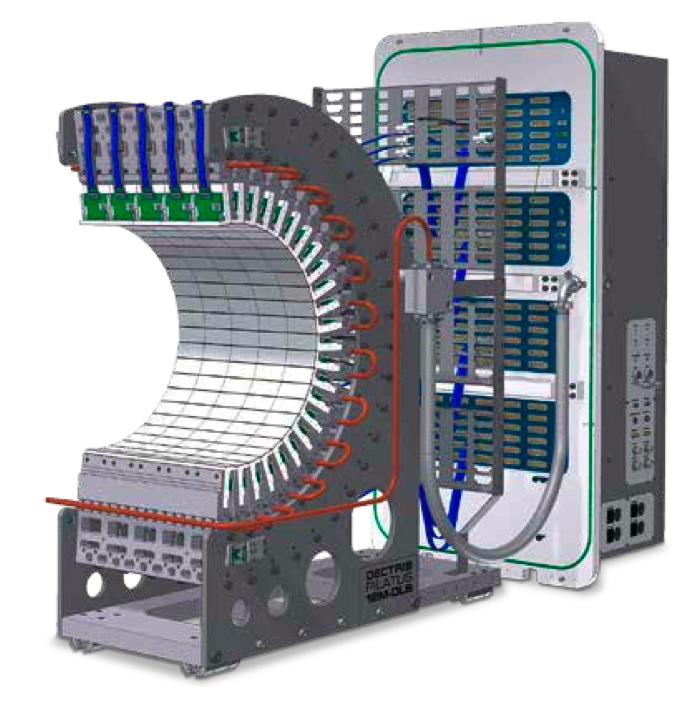
\includegraphics[width=5.5in]{I23.eps}
\label{fig:I23}
\end{figure}

\begin{figure}
\caption{Expected data flows at an NSLS-II beam line with an EIGER X 16M detector.}
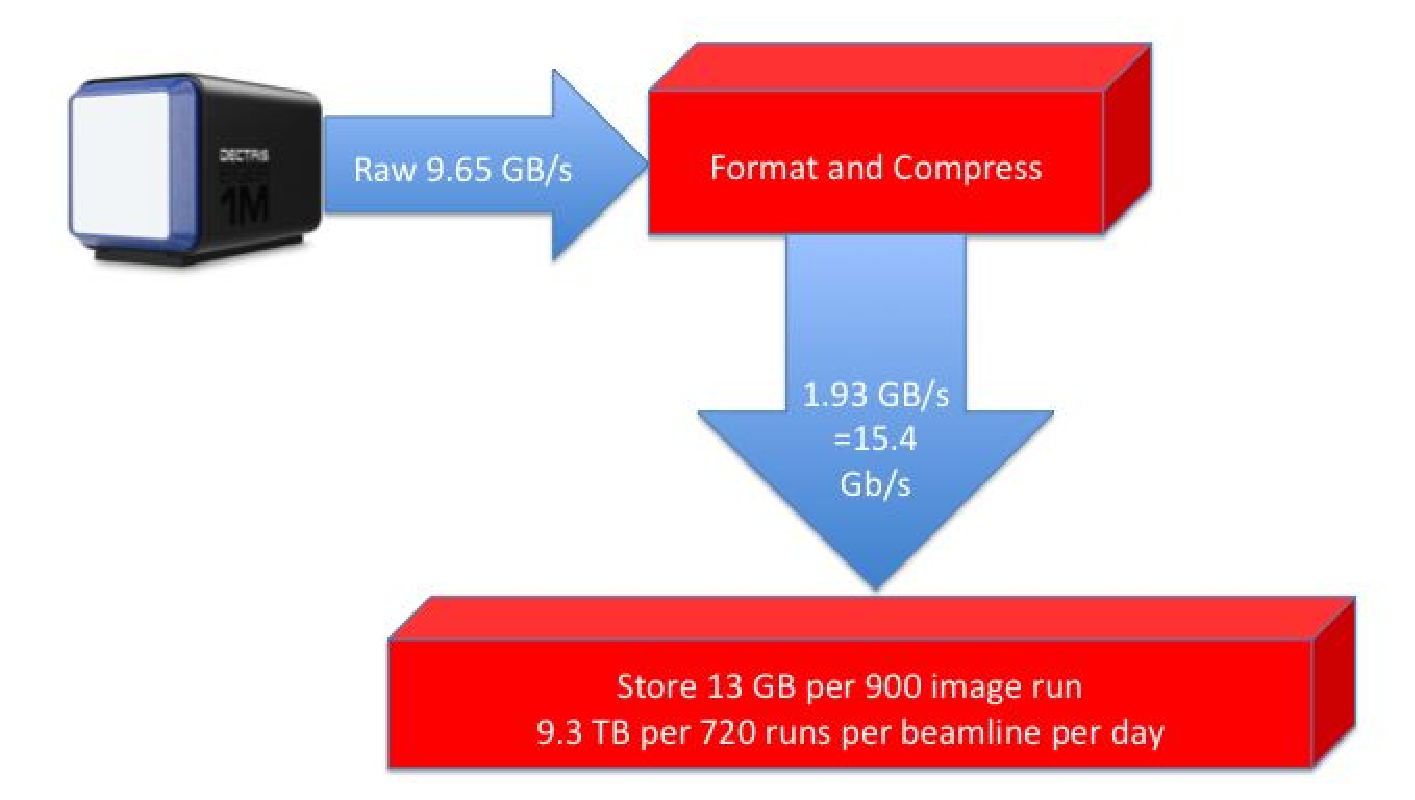
\includegraphics[width=5.5in]{dataflows.eps}
\label{fig:dataflows}
\end{figure}

\begin{table}
\caption{Current compression choices for MX data}
\begin{center}
\begin{tabular}{|l|l|l|l|}  
\hline
{Compression}&{Compression}&{Relative}\\
{Method}&{Ratio}&{Time}\\
\hline
external bzip2 compression&20.4:1 & 5.6\\
HDF5 CBFlib canonical compression &15.7:1 & 3.9 \\
HDF5 CBFlib nibble offset compression 2 Fast 6M&11.5:1 & 2.9 \\
HDF5 CBFlib packed V2 compression 3 6M &11.0:1 & 2.8\\
HDF5 zip compression 16M &9.7:1 & 2.4\\
external LX4 compression (C1 one pass) &8.7:1 & 2.2 \\
HDF5 CBFlib packed compression &8.6:1 &2.2 \\
external LX4 compression (C0 2 passes) &5.2:1&1.3\\
HDF5 CBFlib byte offset compression&4.0:1 &1.0\\
\hline
\end{tabular}
\end{center}
\label{tab:2}
\end{table}

\begin{figure}
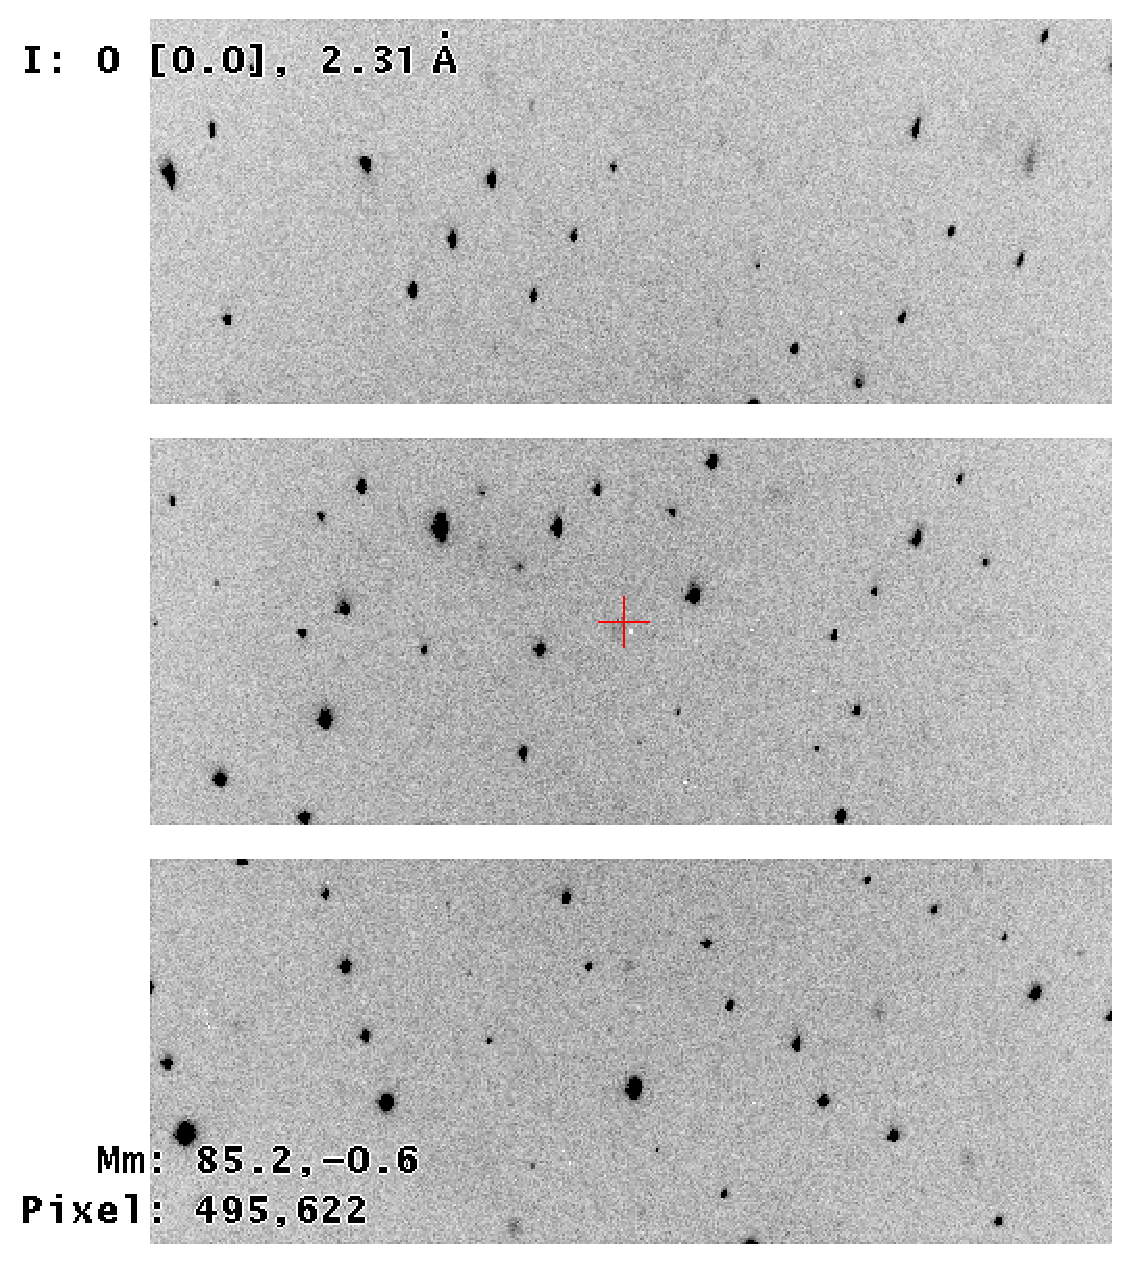
\includegraphics[width=5.5in]{1191_00005.eps}
\label{fig:1191_00005}
\caption{DECTRIS Pilatus 300K image }
\end{figure}


\begin{table}
\label{tab:1191_00005}
\caption{Compressions of a DECTRIS Pilatus 300K image Fig \ref{fig:1191_00005}}
\begin{center}
\begin{tabular}{|l|r|r|}
\hline
{\bf Compression}&{\bf CBF size (MB)}&{\bf HDF5 size (MB)}\\
\hline
raw binary&1.212&1.296\\
byte offset&0.309&0.393\\
HDF5 zlib& n/a &0.370\\
nibble offset&0.207&0.290\\
packed&0.184&0.267\\
canonical&0.178&0.262\\
external bzip2&0.164&0.169\\
\hline
\end{tabular}
\end{center}
\end{table}






\end{document}                    % DO NOT DELETE THIS LINE
%%%%%%%%%%%%%%%%%%%%%%%%%%%%%%%%%%%%%%%%%%%%%%%%%%%%%%%%%%%%%%%%%%%%%%%%%%%%%%
